
		%results
		\begin{figure}[!ht]
		\begin{center}
		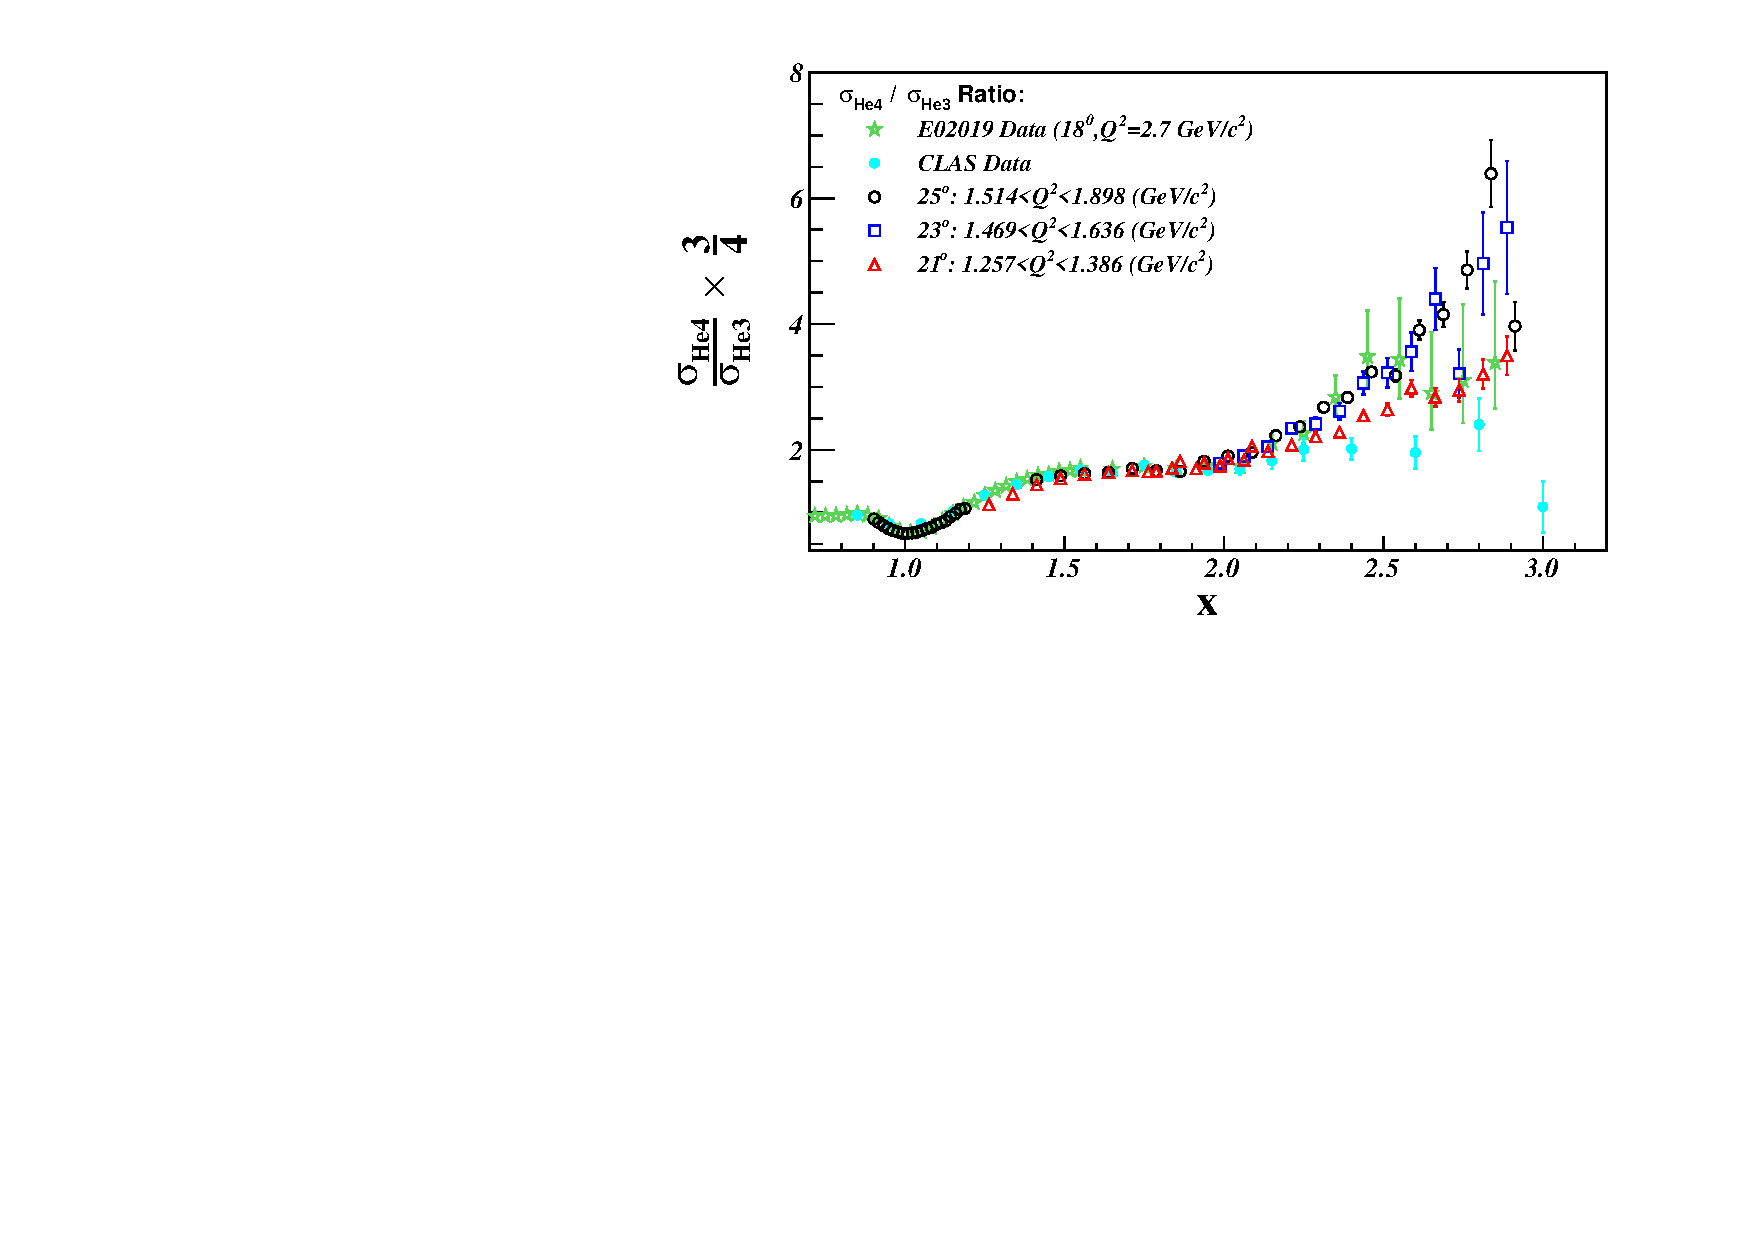
\includegraphics[width=8.0cm]{./figures/He4_He3_XS_Ratio_DpTh40_DpTh40_L.pdf}
		\end{center}
		\vspace*{-5mm}
		\caption{Cross section ratio of $^{4}He$ to $^{3}He$ with this experiment at three $Q^{2}$ settings and also the results from E02-019 and CLAS. Statistical errors and systematic errors from instruments are included.}
		\label{he4_he3}
		\end{figure}
		Fig.~\ref{he4_he3} gives the cross section ratio of $\mathrm{^{4}He}$ to $\mathrm{^{3}He}$ as a function of x. In the 2N-SRC region, the new data reveals a plateau which agrees nicely with the CLAS and E02-019 results. However, at $x>2$, our result shows no 3N-SRC plateau which was claimed by the CLAS data, but instead, raises up quickly when $x$ approaches 3 which tends to agree more with the E02-019 data despite its large errors. While E02-019 ran at higher $\mathrm{Q^{2}}$, the situation becomes interesting that our data and the CLAS data were taken with the similar $\mathrm{Q^{2}}$ range but yield different approaches, and it is ergent to be investigated further. A recent publication suggested that the 3N-SRC plateau showed in the CLAS data could be just a result of inappropriate binning and bin-centering correction~\cite{doug_or_clas}. 

		\begin{figure}[!ht]
		\begin{center}
		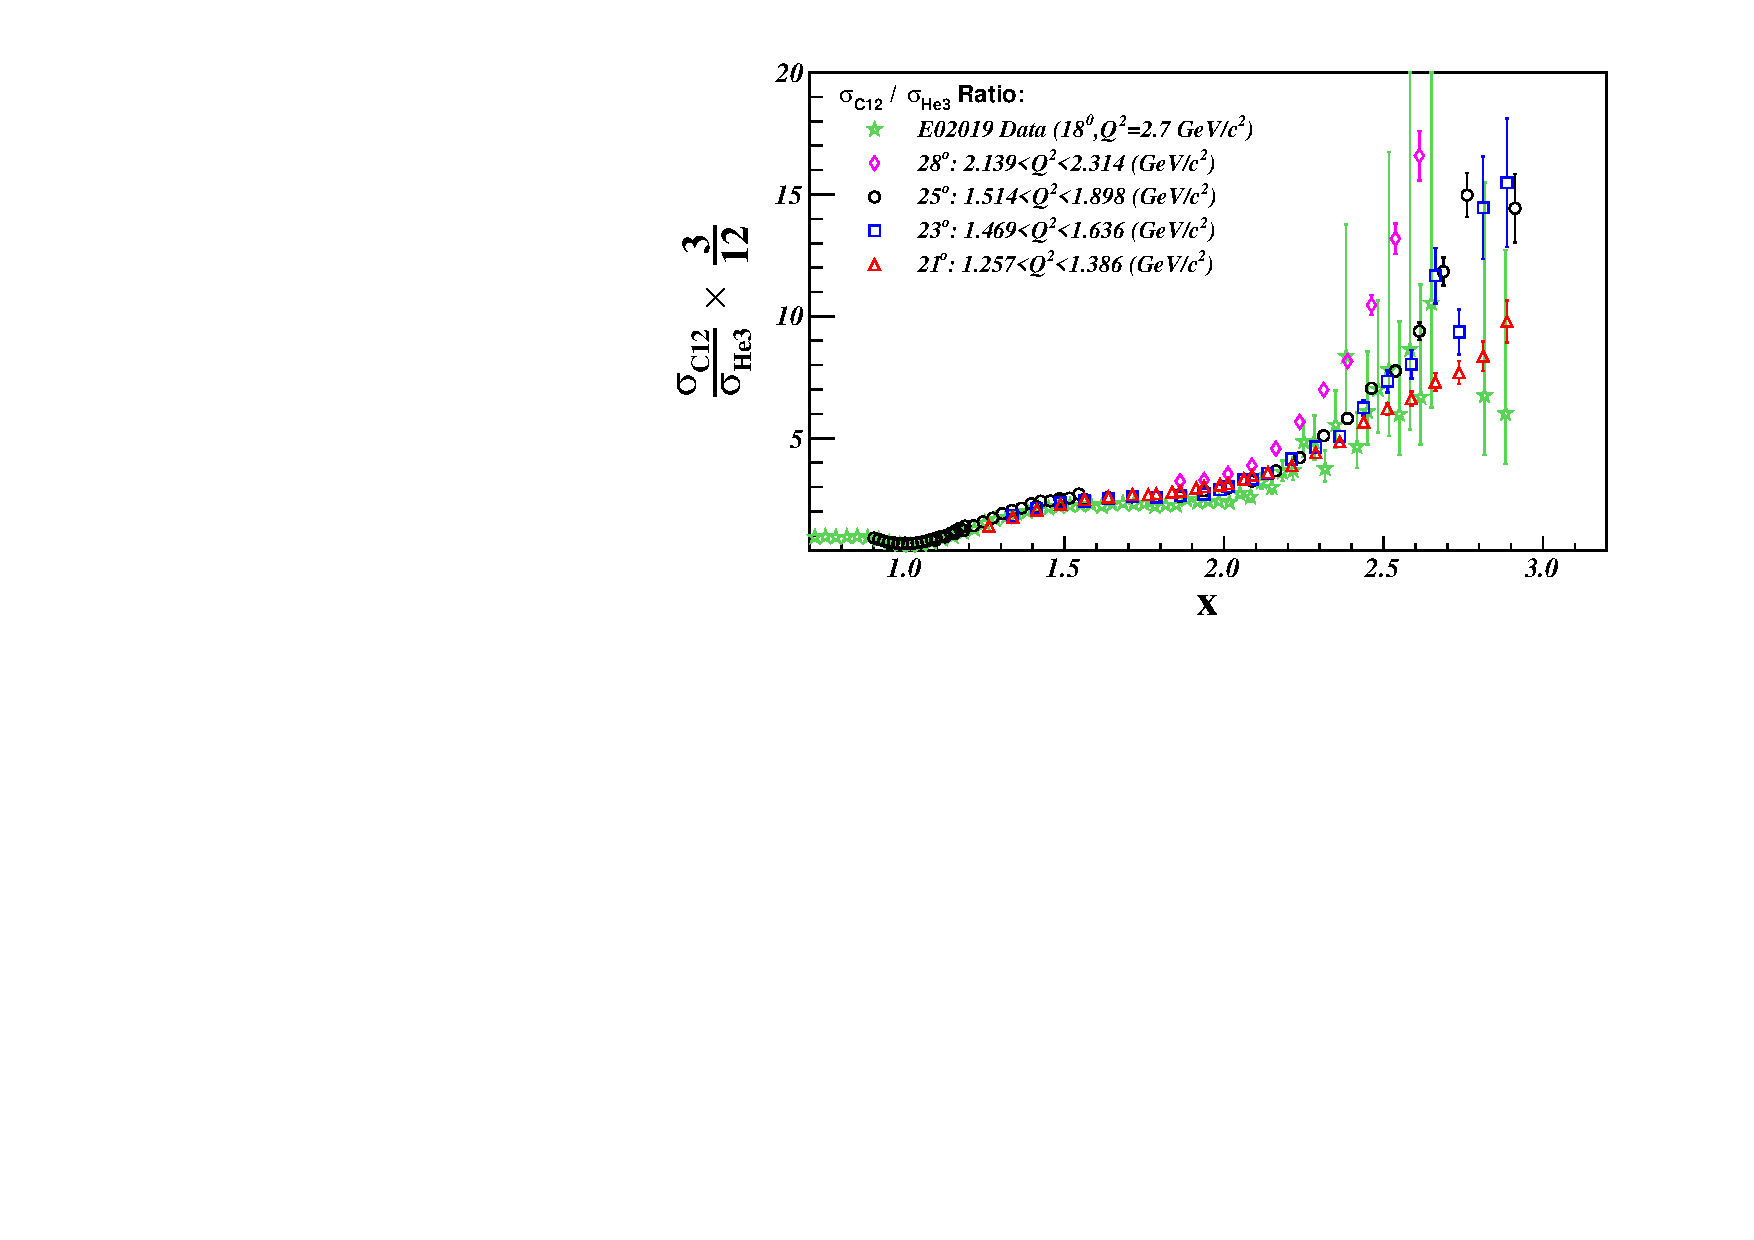
\includegraphics[width=8.0cm]{./figures/C12_He3_XS_Ratio_DpTh40_DpTh40_L.pdf}
		\end{center}
		\vspace*{-5mm}
		\caption{Cross section ratio of $^{12}C$ to $^{3}He$ with this experiment at three $Q^{2}$ settings and also the results from E02-019. Statistical errors and systematic errors from instruments are included.}
		\label{c12_he3}
		\end{figure}
		We also present the new results of the $^{12}C$ to $^{3}He$ ratio and the $^{12}C$ to $^{4}He$ ratio, as shown in Fig.~\ref{c12_he3} and Fig.~\ref{c12_he4}, respectively. The E02-19 result of the $^{12}C$ to $^{3}He$ ratio is also included for comparing. The 2N-SRC plateaus are shown in both plots where there are no indication of the 3N-SRC plateau at large $x$.

		\begin{figure}[!ht]
		\begin{center}
		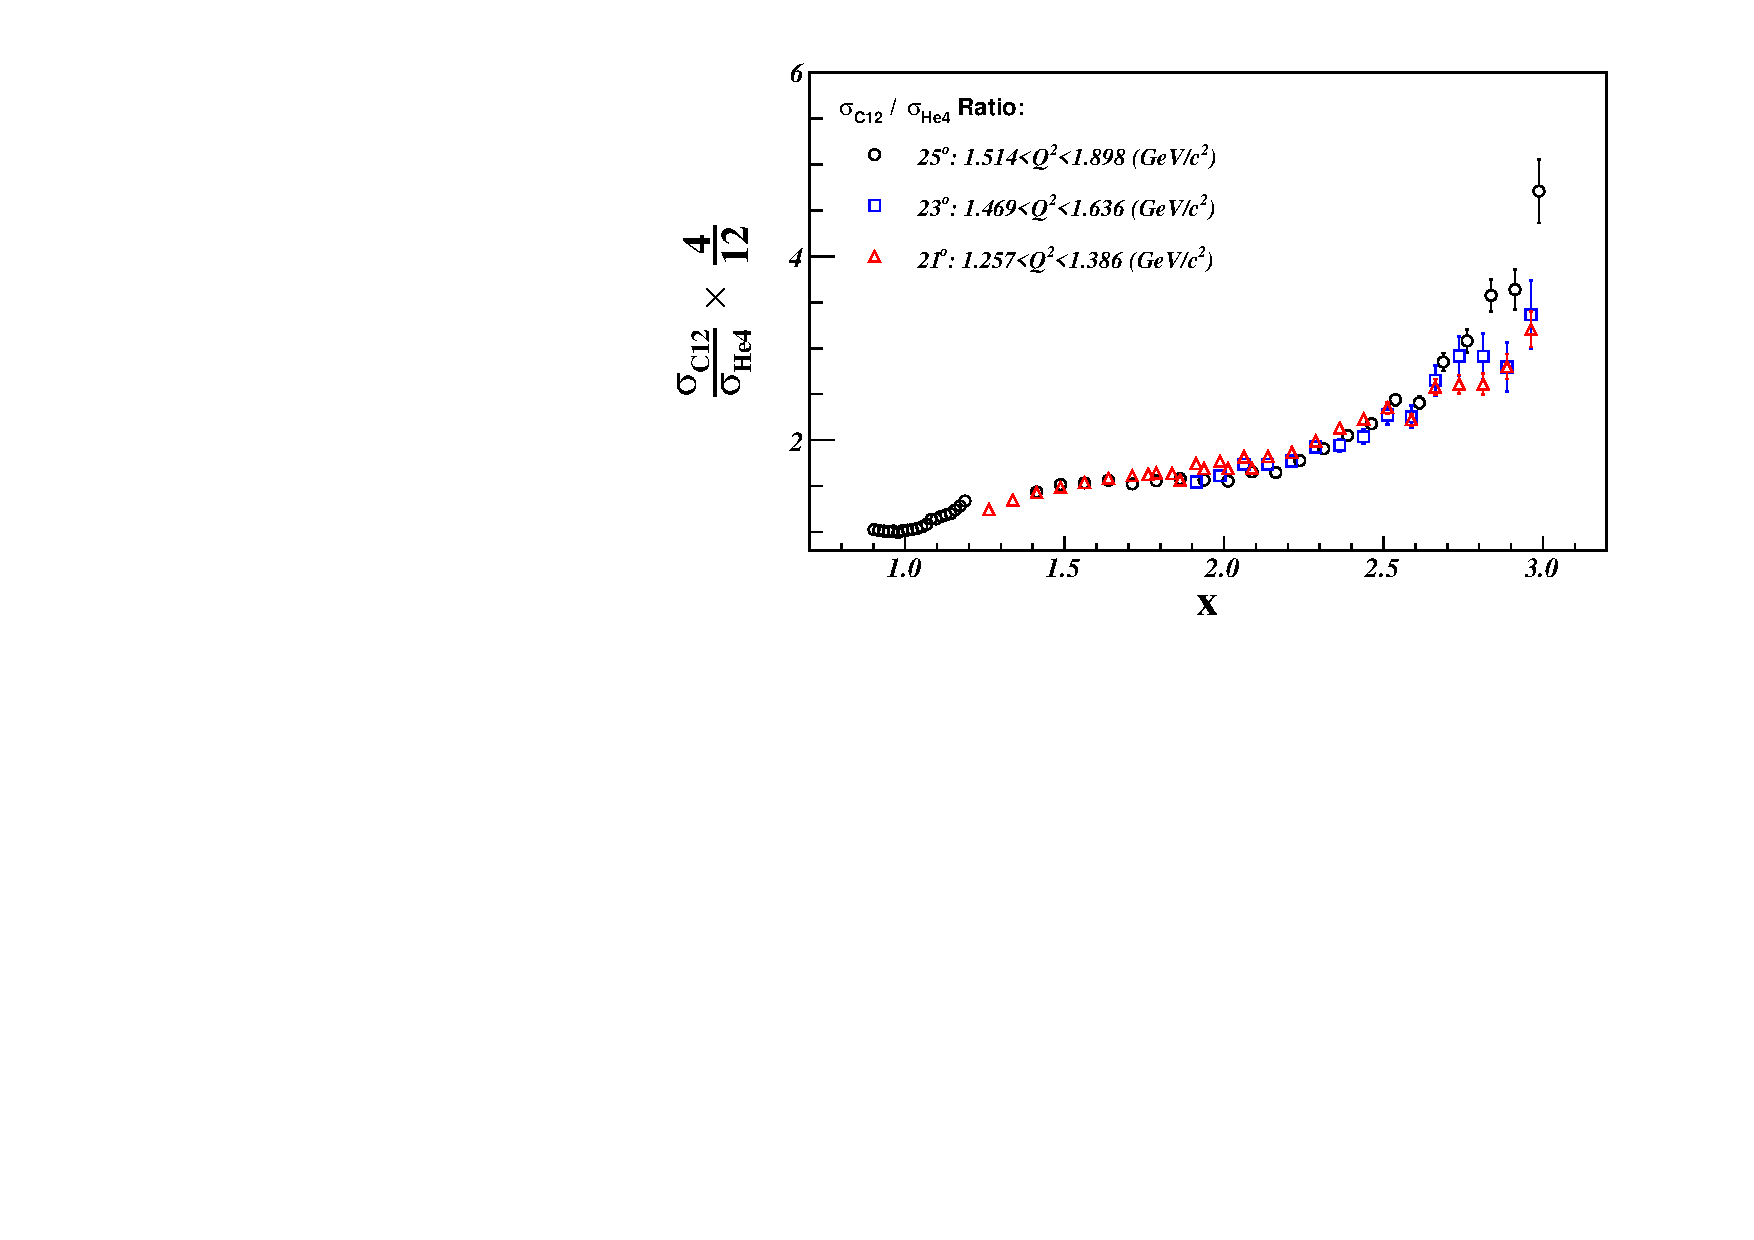
\includegraphics[width=8.0cm]{./figures/C12_He4_XS_Ratio_DpTh40_DpTh40_L.pdf}
		\end{center}
		\vspace*{-5mm}
		\caption{Cross section ratio of $^{12}C$ to $^{4}He$ with this experiment at three $Q^{2}$ settings. Statistical errors and systematic errors from instruments are included.}
		\label{c12_he4}
		\end{figure}


		\begin{figure}[!ht]
		\begin{center}
		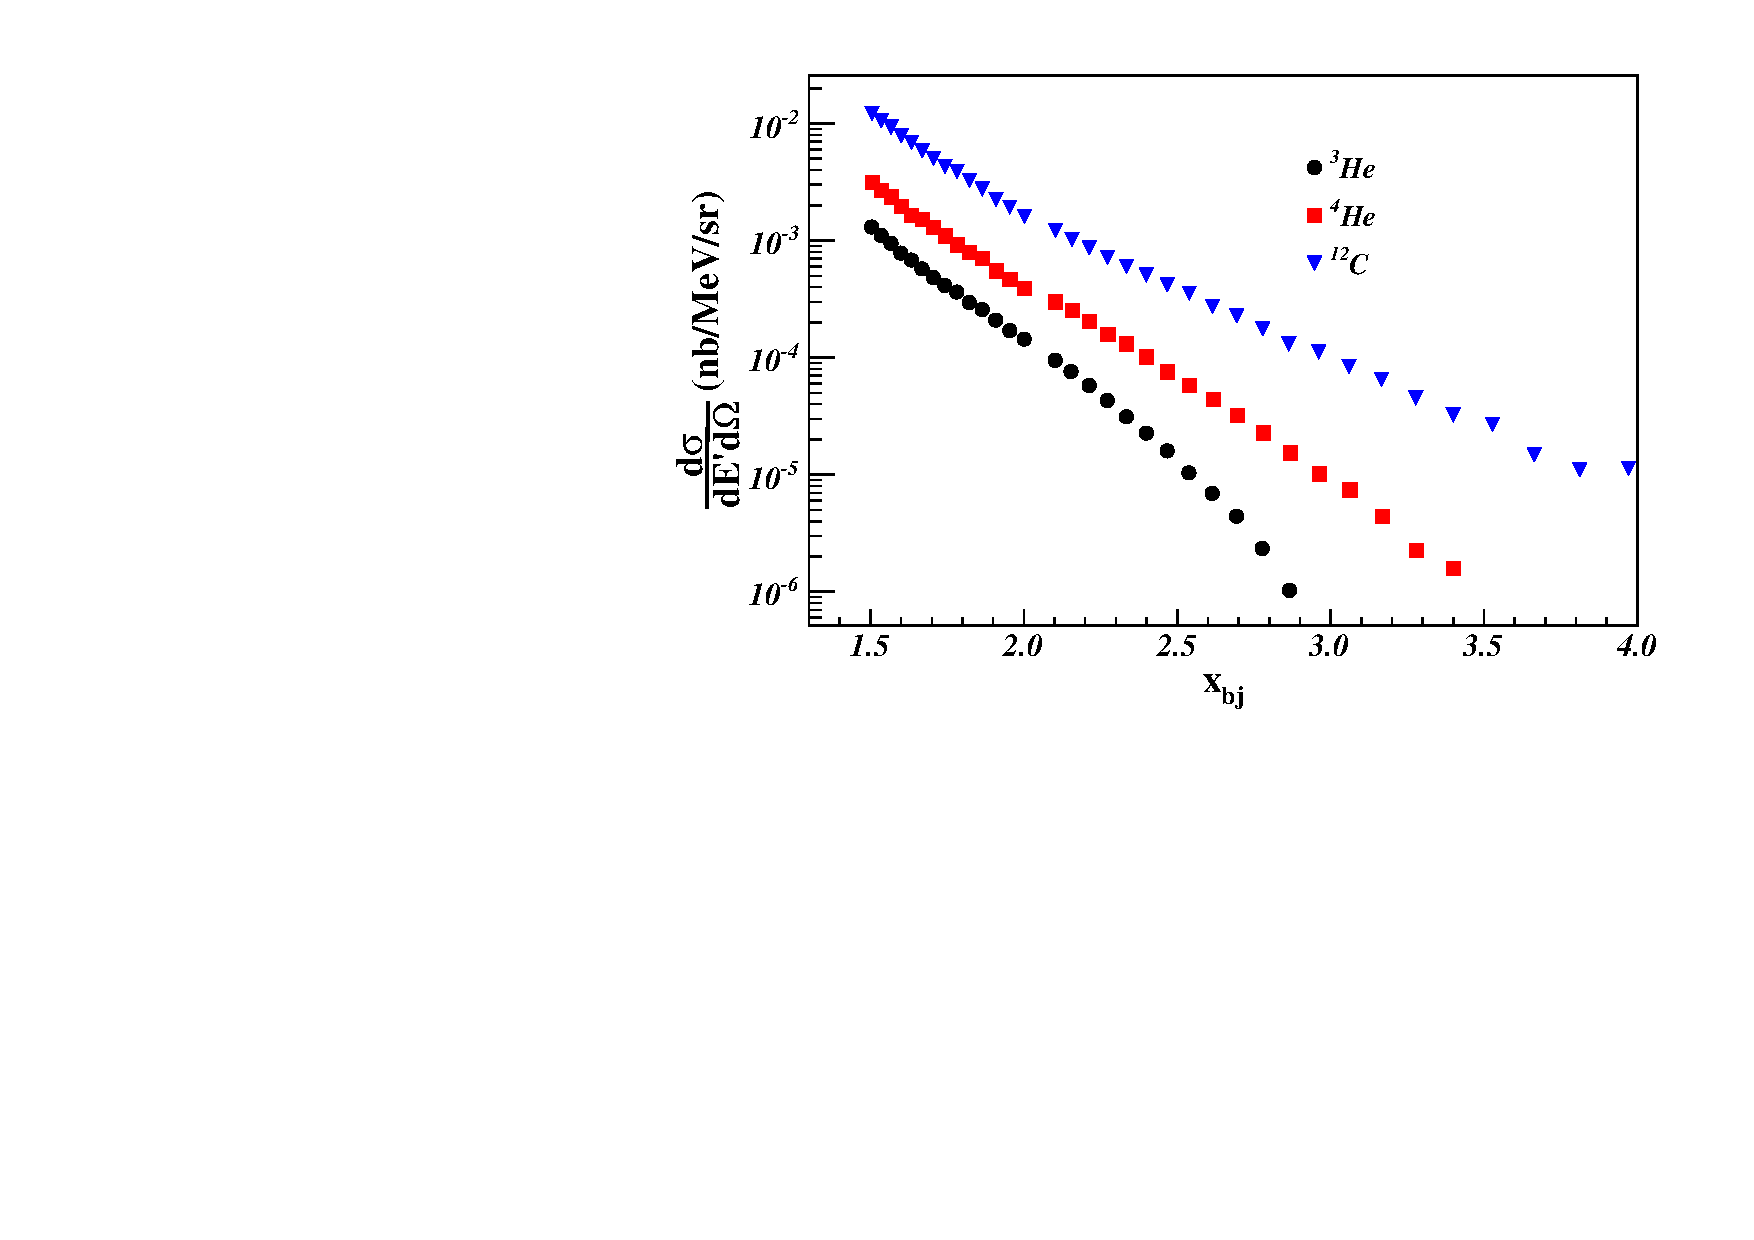
\includegraphics[width=8.0cm]{./figures/XS_Comp_25.pdf}
		\end{center}
		\vspace*{-5mm}
		\caption{Cross sections of $^{3}He$, $^{4}He$ and $^{12}C$ at the $25^{\circ}$ setting. Statistical errors and systematic errors from instruments are included.}
		\label{c12_he4}
		\end{figure}
